%% Seção 3: A Linguagem Atua sobre o Estado Emocional como uma Força Modeladora

\chapter{A Linguagem Atua sobre o Estado Emocional como uma Força Modeladora}

\epigrafe{Os afetos determinam a potência de agir do corpo e, consequentemente, a potência de pensar da mente.}{Baruch Spinoza, \textit{Ética}}

\textbf{3.} A linguagem atua sobre o estado emocional como uma força modeladora, permitindo ao indivíduo nomear e compreender seus afetos, promovendo a autonomia e a autenticidade.

\section{O estado emocional como processo dinâmico}

\textbf{3.1} O estado emocional, sendo um processo dinâmico, é continuamente moldado pela linguagem e pela capacidade de nomear os afetos.

\begin{tese}
Se a linguagem é o meio pelo qual nomeamos e compreendemos nossos afetos (conforme Spinoza), então ela atua diretamente sobre o estado emocional, moldando-o.
\end{tese}

\begin{hipotese}[title=Hipótese 3.1.1 (Condicional)]
Se nomeamos nossos afetos através da linguagem, então podemos compreender e regular nosso estado emocional.
\end{hipotese}

\begin{referencia}[title=Referência a Spinoza]
Para Spinoza, compreender os afetos é essencial para aumentar nossa potência de agir e alcançar a liberdade emocional.
\end{referencia}

\begin{aforismo}
Nomear o sentir é o primeiro passo para dominar o que se sente.
\end{aforismo}

\section{A metáfora como ferramenta de transposição}

\textbf{3.11} A metáfora é uma ferramenta de transposição do estado emocional para a estrutura discursiva, facilitando a compreensão profunda dos afetos.

\begin{tese}
Se a metáfora permite expressar emoções complexas de forma acessível, então ela é um instrumento poderoso na modelagem do estado emocional.
\end{tese}

\begin{hipotese}[title=Hipótese 3.2.1 (Abdução)]
Se o uso de metáforas facilita a expressão e compreensão de emoções profundas, a melhor explicação é que elas ajudam a reorganizar e processar esses afetos.
\end{hipotese}

\begin{aforismo}
A metáfora veste a emoção com palavras que o coração compreende.
\end{aforismo}

\section{Expressão do incomunicável através de metáforas}

\textbf{3.12} O uso de metáforas na linguagem permite que o paciente expresse o que é, de outra forma, incomunicável, avançando em direção à autonomia de existir.

\begin{referencia}[title=Referência a Habermas]
A ação comunicativa autêntica, enriquecida pelo uso de metáforas, facilita o entendimento mútuo e a construção de significados compartilhados.
\end{referencia}

\begin{aforismo}
Na metáfora compartilhada, encontra-se a ponte entre o sentir e o entender.
\end{aforismo}

\section{O estado emocional como curva temporal}

\textbf{3.2} O estado emocional pode ser entendido como uma curva ao longo do tempo, onde a linguagem é o vetor que define sua forma, permitindo a transformação através da nomeação dos afetos.

\begin{tese}
Se a linguagem influencia a trajetória emocional ao longo do tempo, então reestruturar a linguagem permite modificar o estado emocional.
\end{tese}

\begin{hipotese}[title=Hipótese 3.3.1 (Condicional)]
Se alteramos a forma como expressamos nossos afetos através da linguagem, então podemos alterar a evolução de nosso estado emocional.
\end{hipotese}

\begin{aforismo}
A palavra renascida transforma o caminho do sentir.
\end{aforismo}

%% DIAGRAMA: Curva Emocional
\begin{center}
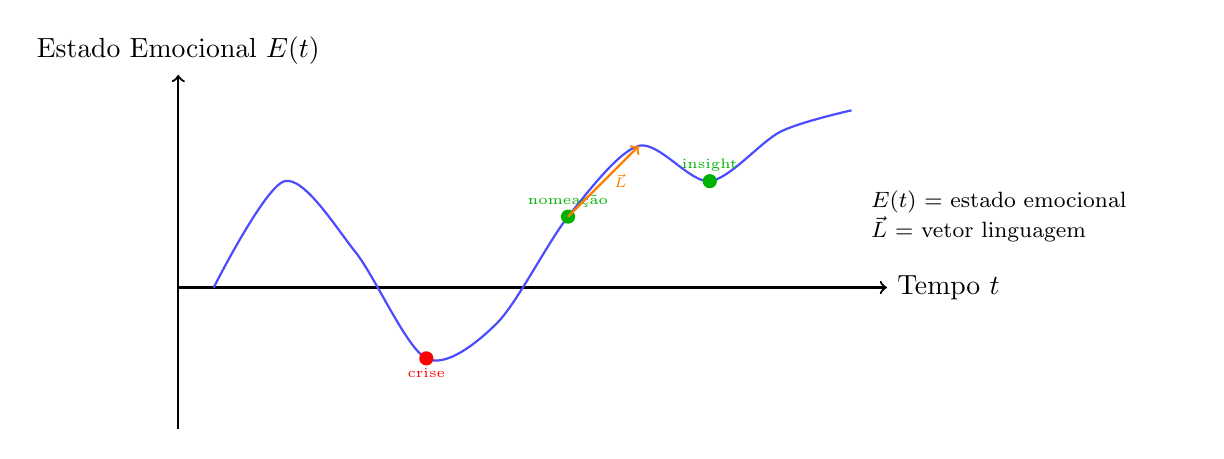
\begin{tikzpicture}[scale=0.9]
    % Eixos
    \draw[thick, ->] (0,0) -- (10,0) node[right] {Tempo $t$};
    \draw[thick, ->] (0,-2) -- (0,3) node[above] {Estado Emocional $E(t)$};

    % Curva emocional
    \draw[thick, blue!70, smooth] plot coordinates {(0.5,0) (1.5,1.5) (2.5,0.5) (3.5,-1) (4.5,-0.5) (5.5,1) (6.5,2) (7.5,1.5) (8.5,2.2) (9.5,2.5)};

    % Pontos de inflexão (intervenção linguística)
    \fill[red] (3.5,-1) circle (0.1) node[below, font=\tiny] {crise};
    \fill[green!70!black] (5.5,1) circle (0.1) node[above, font=\tiny] {nomeação};
    \fill[green!70!black] (7.5,1.5) circle (0.1) node[above, font=\tiny] {insight};

    % Vetor da linguagem
    \draw[thick, ->, orange] (5.5,1) -- (6.5,2) node[midway, right, font=\tiny] {$\vec{L}$};

    % Legenda
    \node[font=\footnotesize, text width=4cm] at (12,1) {$E(t)$ = estado emocional\\$\vec{L}$ = vetor linguagem};
\end{tikzpicture}
\end{center}

\section{Narrativas e metáforas na organização emocional}

\textbf{3.3} Quando o paciente expressa emoções através de narrativas e metáforas, ele transita de um estado caótico para um estado organizável, construindo seu self e compreendendo seus valores pessoais.

\begin{tese}
Se a narrativa organiza o caos emocional, então contar e recontar a própria história é um processo de construção do self e de autonomia.
\end{tese}

\begin{hipotese}[title=Hipótese 3.4.1 (Condicional)]
Se o paciente elabora narrativas coerentes sobre suas experiências emocionais, então ele promove a organização interna e a compreensão de seus valores.
\end{hipotese}

\begin{referencia}[title=Referência a Habermas]
A ação comunicativa na forma de narrativas compartilhadas permite a construção de identidades e significados pessoais.
\end{referencia}

\begin{aforismo}
Na história que se conta, o eu se descobre e se afirma.
\end{aforismo}

\section{Rastreamento de variações emocionais}

\textbf{3.4} As variações emocionais podem ser rastreadas através da análise contínua da linguagem; assim, a linguagem atua como um barômetro dos afetos e um guia para a autonomia.

\begin{tese}
Se a linguagem reflete as variações emocionais, então seu monitoramento permite compreender e regular os afetos ao longo do tempo.
\end{tese}

\begin{aforismo}
A palavra que muda revela o sentir que se transforma.
\end{aforismo}

%% DIAGRAMA COMPLETO DA SEÇÃO 3
\section*{Diagrama Representativo: Linguagem como Força Modeladora}

\begin{center}
\begin{tikzpicture}[scale=1, every node/.style={font=\small}]
    % Estado Emocional como processo
    \node[draw, ellipse, fill=red!20, minimum width=3cm, minimum height=1.5cm] (emo) at (0,3) {Estado Emocional};

    % Linguagem
    \node[draw, rectangle, rounded corners, fill=green!30, minimum width=4cm, text width=3.5cm, align=center] (ling) at (0,0) {Linguagem\\(Metáforas, Narrativas)};

    % Processo de nomeação
    \node[draw, diamond, fill=purple!20, aspect=2, text width=2cm, align=center, font=\tiny] (nom) at (-4,1.5) {Nomeação\\dos Afetos\\(Spinoza)};

    % Ação comunicativa
    \node[draw, diamond, fill=orange!20, aspect=2, text width=2cm, align=center, font=\tiny] (acao) at (4,1.5) {Ação\\Comunicativa\\(Habermas)};

    % Setas de influência
    \draw[thick, <->, blue!70] (emo) -- node[left, font=\tiny] {modela} (ling);
    \draw[thick, ->] (nom) -- (emo);
    \draw[thick, ->] (nom) -- (ling);
    \draw[thick, ->] (acao) -- (emo);
    \draw[thick, ->] (acao) -- (ling);

    % Resultado
    \node[draw, rounded corners, fill=teal!30, text width=4cm, align=center] (result) at (0,-2.5) {Autonomia, Autenticidade\\e Transformação Emocional};

    \draw[thick, ->] (ling) -- (result);

    % Curva temporal à direita
    \begin{scope}[shift={(7,0)}]
        \draw[thick, ->] (0,-2) -- (0,4) node[above, font=\tiny] {$E(t)$};
        \draw[thick, ->] (0,0) -- (3,0) node[right, font=\tiny] {$t$};
        \draw[thick, blue!70, smooth] plot coordinates {(0.2,0) (0.8,1.5) (1.4,0.5) (2,2) (2.6,2.5)};
        \node[font=\tiny] at (1.5,-2.5) {Trajetória Emocional};
    \end{scope}
\end{tikzpicture}
\end{center}

\begin{sintese}[title=Síntese Final da Seção 3]
A linguagem atua sobre o estado emocional como uma força modeladora, permitindo ao indivíduo nomear e compreender seus afetos, o que é essencial para a autonomia e a autenticidade do ser. Conforme Spinoza, a compreensão dos afetos aumenta a potência de agir; ao nomeá-los através da linguagem, especialmente utilizando metáforas e narrativas, o paciente pode transpor emoções complexas para uma estrutura compreensível, facilitando sua gestão e transformação.

A metáfora emerge como uma ferramenta poderosa para expressar o incomunicável, permitindo que o paciente avance em direção à autonomia de existir. A narrativa organiza o caos emocional, possibilitando ao indivíduo construir seu self e compreender seus valores pessoais. A análise contínua da linguagem atua como um barômetro dos afetos, permitindo rastrear variações emocionais e intervir de forma eficaz.
\end{sintese}

\nextpage
